\chapter{Fussballszenario} \label{kap:Fussballszenario} %TODO: Besseren Kapiteltitel

\section[Szenario Koordination]{Szenario Koordination\hfill {\normalsize H.O.}} \label{sec:szenario_koordination}

Die Szenario Koordination umfasst sowohl das Verhalten der einzelnen AMiRos, kooperative Elemente zwischen verschiedenen AMiRos, als auch die Kommunikation mit dem Host-PC. Der Entwurf dieser drei Themenbereiche soll im folgenden kurz vorgestellt und begründet werden:

Um ein bestimmtes Verhalten zu zeigen, müssen die AMiRos selbst zunächst über einen Satz einzelner Fähigkeiten verfügen. Ein komplexeres Verhalten entsteht dann aus der Kombination der einzelnen Fähigkeiten, indem diese sequenziell oder parallel miteinander kombiniert werden. Denkbar wäre ebenso die Realisierung einer Verhaltenshierarchie, in der sich einzelne Verhaltensweisen beeinflussen und sich gegenseitig unterdrücken oder verstärken können. Ein solcher Ansatz wird näher in \cite{Brooks:1986} beschrieben.

Da das Szenario in seiner Komplexität jedoch noch begrenzt ist und kein vollständig generisches Verhalten implementiert werden musste, wurde die Umsetzung im Projektkontext durch einen endlichen Automaten / eine (Finite-)State-Machine realisiert. Die Zustände stellen einzelne Verhaltensweisen des Roboters dar und durch bestimmte Nachrichten (Events) kann zwischen ihnen gewechselt werden.

Das Verhalten einzelner AMiRos wird erweitert durch kooperative Fähigkeiten und die Möglichkeit der Kommunikation durch einen festgelegten Befehlssatz. Kann beispielsweise ein AMiRo während einer Spielaktion den Ball nicht lokalisieren, kann er eine Nachricht an den anderen AMiRo schicken, woraufhin dieser sich dann ein Stück bewegt, um die Sicht auf den Ball freizugeben.

Zusätzlich besteht die Möglichkeit für die AMiRos mit dem Host-PC zu kommunizieren, welcher an Hand eines Kamerabildes und zusätzlicher Bildverarbeitungslogik das Spielgeschehen verfolgen, interpretieren und steuern kann. Dies erlaubt außerdem eine Benutzerinteraktion, um das Spiel zu starten, zu pausieren oder zu unterbrechen. In der derzeitigen Realisierung übermittelt der Host-PC außerdem noch den Status des Spielballs, also ob dieser in Bewegung ist oder ruht. Diese Information wird von den AMiRos verwendet, um eigenständig zu bestimmen, welcher AMiRo gerade am Zug ist.

\section[Kommunikation per RSB und Spread]{Kommunikation per RSB und Spread\hfill {\normalsize H.O.}}
Damit die AMiRos untereinander kommunizieren können, wurde eine Publish-Subscribe Architektur basierend auf der RSB Middleware aufgesetzt und anstatt einer einfachen Socket-Transport Lösung wurde auf das etwas komplexere Spread Toolkit zurückgegriffen (siehe RSB Konfigurationsdatei im Anhang \ref{sec:rsb-config}).

Die Publish-Subscribe Architektur bietet den Vorteil der asynchronen Kommunikation, die im Zusammenspiel mit einer State-Machine besonders praktisch ist. Die State-Machine muss nicht auf explizit auf Antworten warten, sondern kann beliebig weiterlaufen und schaut in jedem Zyklus, ob neue Nachrichten empfangen wurden. Zudem bietet sie den Vorteil, dass sehr leicht Software-Komponenten hinzugefügt und an die bestehende Kommunikation angeschlossen werden können (vgl.\cite{Siciliano:2007}).

Jeder AMiRo (und auch der Host-PC) hat also eine bestimmte Anzahl an Empfängern (Listener) und Sendern (Publisher) um Nachrichten in bestimmten Geltungsbereichen (Scopes) zu empfangen oder zu senden. Als Nachrichten werden der Einfachheit halber einfache Strings versendet, die dann beim Empfänger geparst werden können. Das Debugging während der Entwicklung wurde so vereinfacht, allerdings hat dieser Ansatz auch Nachteile: Zum einen müssen die Listen an Strings auf Empfänger und Senderseite immer gepflegt werden, damit sie identisch sind und ein zuverlässiges Parsen erlauben. Zum anderen bieten gekapselte Nachrichten mehr Typensicherheit und ggf. auch die Option zusammengehörige Informationen zu kapseln. Im Umfang des Projekt war die Wahl lediglich einfach Strings zu übertragen durchaus ausreichend, die Lösung skaliert aber nicht zwingend für größere Projekte.

Das Spread Toolkit hilft dabei einen Nachteil der allgemeinen Publish-Subscriber Architektur zu beseitigen: Die Kommunikation beruht nicht auf einem zentralen Endpunkt, der die gesamte Kommunikation steuert, sondern jeder Spread-Daemon überwacht die Verbindungen zu allen anderen Endpunkten und hält diese so aufrecht (vgl.\cite{Siciliano:2007}). So kann auch bei kurzzeitigen Verbindungsabbrüchen sichergestellt werden, dass die Verbindung automatisch wiederhergestellt wird. Auf Programmebene  muss so weniger Overhead für die Sicherstellung der Verbindung implementiert werden und der Code bleibt einfacher und somit besser wartbar.

Neben der Plattform-übergreifenden Kommunikation werden RSB und Spread zusätzlich auch für Interprozess-Kommunikation auf den AMiRos und auf dem Host-PC eingesetzt. Wie in Abb. \ref{fig:spread} zu sehen ist, laufen auf beiden AMiRos die drei gleichen Softwarekomponenten. Die State-Machine (\texttt{FSM}) steuert das Verhalten und die Kommunikation. Die \texttt{locateAndShoot} Komponente stellt die Verhaltenseinheiten für das Szenario zur Verfügung und die \texttt{SearchCharging} Komponente erlaubt aus dem Szenario aus die Lokalisation und das Anfahren an die Ladestation. Diese drei Komponenten kommunizieren über den internen Spread, der auf der internen Localhost Schnittstelle auf dem Port 4806 läuft (siehe dazu auch Anhang \ref{sec:spread-config}).

Die Kommunikation zwischen den AMiRos selbst und dem Host läuft über einen weiteren Spread-Daemon, der mit einer anderen Konfiguration geladen wird, die W-LAN Schnittstelle nutzt und auf Port  4803 hört und sendet (siehe ebenfalls Abschnitt \ref{sec:spread-config}).

Die W-LAN Verbindung wurde durch einen eigenen Router realisiert und erlaubt so die feste Adresszuweisung für die drei Endpunkte, damit die Spread-Konfiguration darauf zurückgreifen kann. Die Einzelheiten können der W-LAN Konfiguration im Anhang (Abschnitt \ref{sec:wlan-config}) entnommen werden.
\begin{figure}
	\begin{center}
		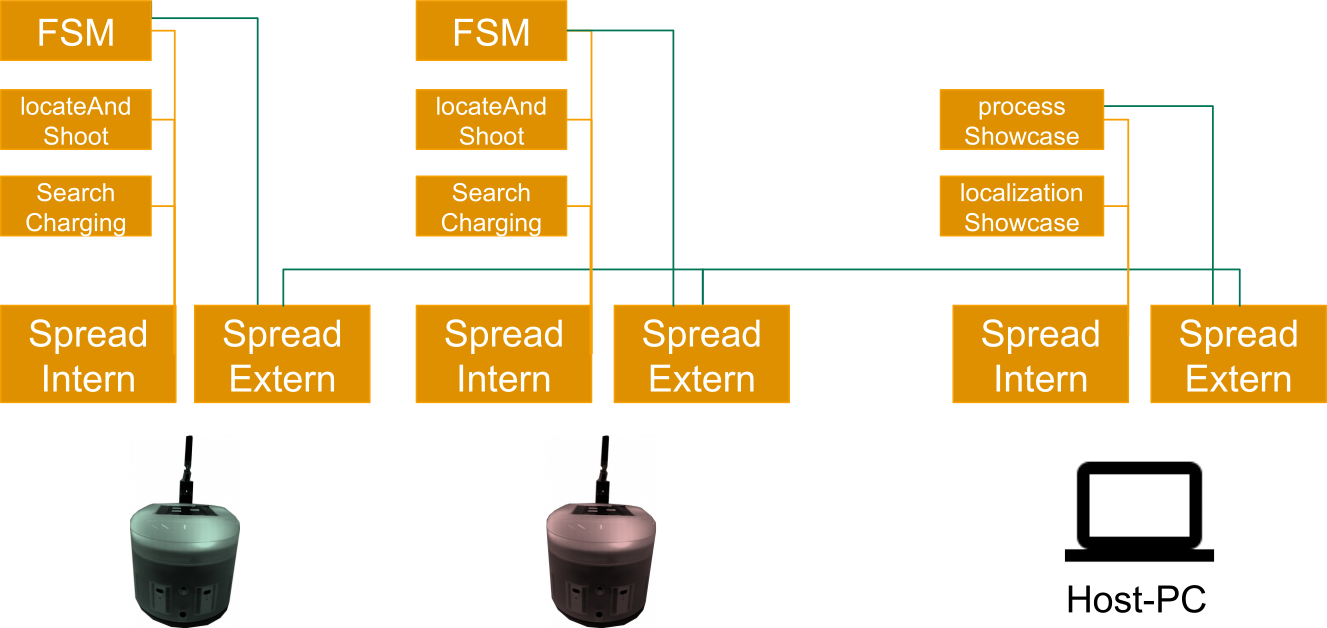
\includegraphics[scale=.65]{spread_communication.png} 	
		\caption{Spread-Kommunikation}
		\label{fig:spread}
	\end{center}
\end{figure}


\subsection[Finite-State-Machine]{Finite-State-Machine\hfill {\normalsize H.O.}}
Die State-Machine regelt das Verhalten der einzelnen AMiRos. Jedes Verhalten wird in kleinstmögliche Einheiten unterteilt, die dann einzeln angesprochen und überall wiederverwendet werden können. Nach der Initialisierung aller RSB-Komponenten und Variablen wird im Programm die State-Machine gestartet.

Solange kein Fehler auftritt, bleibt das Programm immer innerhalb der State-Machine und wechselt den aktuellen Zustand nur auf Grund externer Nachrichten, die in Form von RSB Events oder CAN Messages eingehen können. Extern beschreibt also in diesem Zusammenhang sowohl die anderen Programmkomponenten die auf dem AMiRo laufen, als auch RSB Events von einem anderen AMiRo oder dem Host-PC und CAN Nachrichten vom Mikrocontroller.

Einzelne Zustände haben auch direkte Anweisungen, die den aktuellen Zustand wechseln können, dies soll eine Kapselung der einzelnen Verhaltenseinheiten unterstützen und erlaubt so zukünftige Änderungen oder Erweiterungen leichter durchführen zu können.

Die State-Machine selbst ist in Abb. \ref{fig:fsm-amiro} dargestellt. Nach dem Start ist zunächst der \texttt{idle} Zustand aktiv. Dieser wartet lediglich auf Kommandos und stellt sicher, dass sich der AMiRo nicht bewegt, sondern ruhig auf seiner Position abwartet.

Um das Spiel zu starten, muss eine Nachricht vom Host-PC an die AMiRos geschickt werden.Der aktuelle Zustand wechselt dann auf \texttt{startScenario}. Hier können Initialisierungen vorgenommen werden, die notwendig sind, damit der Roboter das Spiel antreten kann. In der derzeitigen Implementierung werden beispielsweise die Teamfarben auf den oberen LEDs des AMiRos gesetzt. Eine mögliche Erweiterung des Szenarios wäre beispielsweise, dass die Spieler auch bestimmte Positionen auf dem Spielfeld einnehmen.

Ist die Initialisierung abgeschlossen, wechselt die State-Machine in den \texttt{ready} Zustand. In diesem Zustand bleibt die FSM solange, bis der Host-PC das Spiel offiziell startet, doch abbricht oder bis die Ladestrategie das Ladeverhalten anstößt.

Wird das Spiel gestartet, ist der \texttt{waitForTurn} State aktiv. Dieser wartet im Normalfall auf die Nachricht eines anderen AMiRos, der seinen Spielzug abgeschlossen hat und somit das Handle an ihn selbst übergibt. Beim Spielstart hingegen versendet der Host-PC einmalig ein Event mit entsprechendem Inhalt und definiert so, welche Roboter beginnen darf. Im normalen Spielverlauf kann es auch passieren, dass der AMiRo dem Gegner die Sicht auf den Ball verdeckt. Signalisiert der Gegner dies durch eine Nachricht, wechselt die State-Machine in den \texttt{moveFromBall} State, sendet dort eine Nachricht an die \texttt{locateAndShoot} Anwendung und wechselt dann wieder zurück in den \texttt{waitForTurn} Zustand. Gleichzeitig wird eine Bestätigungsnachricht an den Gegner verschickt um zu signalisieren, dass die Neupositionierung abgeschlossen ist.

Ist der AMiRo selbst an der Reihe, um seinen Spielzug zu machen, beginnt er damit im \texttt{localizeBall} State. Er versucht den Ball zu lokalisieren und wechselt bei erfolglosem Versuch in den \texttt{waitForOtherAmiroMove} Zustand, in dem eine Nachricht an den Gegner geschickt wird, damit dieser sich bewegt. Nach Bestätigung des Gegners, dass dieser seine Position geändert hat, wechselt die FSM wieder in den \texttt{localizeBall} Zustand und versucht erneut die Lokalisierung des Balls. Bei Erfolg wird dann zu \texttt{moveToBall} gewechselt.

Die folgenden Zustände verlaufen sequenziell und können daher zusammenfassend beschrieben werden:
\texttt{moveToBall}, \texttt{findGoal}, \texttt{moveToShootingPosition}, \texttt{shootBall}. Jeder dieser Zustände verschickt ein Event an das \texttt{locateAndShoot} Programm, wartet auf erfolgreiche Rückmeldung und wechselt dann in den jeweils nachfolgenden State. Wie auch in den meisten Zuständen zuvor, gibt es zusätzlich noch die Möglichkeit, dass das Spiel abgebrochen wird oder der AMiRo laden muss. Dann wird jeweils in den \texttt{cancelScenario} oder in den \texttt{moveToEdge} State gewechelt.

Nachdem der Ball vom Roboter geschossen wurde, muss zunächst auf eine Bestätigung vom Host-PC gewartet werden, bis der Ball sich nicht mehr bewegt. Erst dann soll das Handle an den anderen AMiRo übergeben werden. Der Host-PC sendet allerdings kontinuierlich ein Signal aus, solange sich der Ball bewegt, die State-Machine wartet sicherheitshalber mehrere Durchgänge in denen keine Nachricht vom Host-PC empfangen werden darf, die eine Ballbewegung signalisiert. Erst dann wird das Handle im nachfolgenden State \texttt{giveHandleToOtherAmiro} übergeben. In diesem Zustand ist ein Hand-Shaking Mechanismus eingebaut, um sicherzustellen, dass der Gegner das Handle auch empfangen hat. Ist das der Fall, wird wieder zurück in den \texttt{waitForTurn} Zustand gewechselt.

Auch das Ladeverhalten wird aus State-Machine Sicht in mehrere Schritte unterteilt und erlaubt so eine gewisse Flexibilität. Gestartet wird das Ladeverhalten durch den \texttt{moveToEdge} State, der den Roboter aus dem Spielgeschehen heraus lenken soll, bis er die nächste Kante gefunden hat.

Ist er dort angekommen, wechselt er in den \texttt{waitingAtEdge} Zustand. Je nach dem ob die Ladestation gerade frei ist, kann die FSM dann direkt in den nächsten Zustand übergehen oder muss dort solange warten, bis die Ladestation frei wird.

Im \texttt{moveToCharging} Zustand startet der AMiRo eine Kantenverfolgung und versucht dann an Hand bestimmter Merkmale die Ladestation zu lokalisieren, indem er entsprechende RSB Events an die SearchCharging Anwendung sendet.

Ist er an der Ladestation angekommen, wechselt die State-Machine in den\linebreak \texttt{moveIntoStation} State und kommuniziert dann über CAN Nachrichten mit den Mirkocontroller Schnittstellen. Wird ein erfolgreiches Andocken zurückgemeldet, wird dann (ebenfalls über CAN) das eigentliche Laden gestartet. Der Roboter lädt dann in der Regel vollständig auf, es sei denn er empfängt zwischendurch Notrufsignale von einem anderen AMiRo der einen kritischen Ladezustand erreicht hat. 

\subsection[Ladestrategie]{Ladestrategie\hfill {\normalsize H.O.}}
Während des Szenarios ist es für die Roboter wichtig, ihren eigenen Ladezustand zu überwachen und beim Überschreiten gewisser Grenzwerte ein bestimmtes Verhalten auszulösen.

Der aktuelle Ladezustand kann wird bei jedem Durchlauf der FSM über den CAN Bus abgefragt und überprüft. Die genaue Ladestrategie wird in Abb. \ref{fig:charging-strategy} verdeutlicht. Fällt die Ladekapazität unter 10\%  wird zunächst überprüft, welchen Ladezustand der andere AMiRo aktuell hat. Liegt dieser unter 15\%, wird das Ladeverhalten gestartet. Fällt die eigene Ladekapazität unter 5\% wird das Ladeverhalten ebenfalls ausgelöst, unabhängig vom Ladezustand des anderen AMiRos. Wird dann eine weitere Grenze von 2\% unterschritten, wird zusätzlich eine Art Notrufsignal vom AMiRo gesendet. Dieses Signal veranlasst einen anderen Roboter, welcher gerade die Ladestation blockiert, aber schon ein bestimmtes Ladelevel erreicht hat, seinen Ladevorgang abzubrechen und die Ladestation frei zu machen.

\begin{figure}
	\begin{center}
		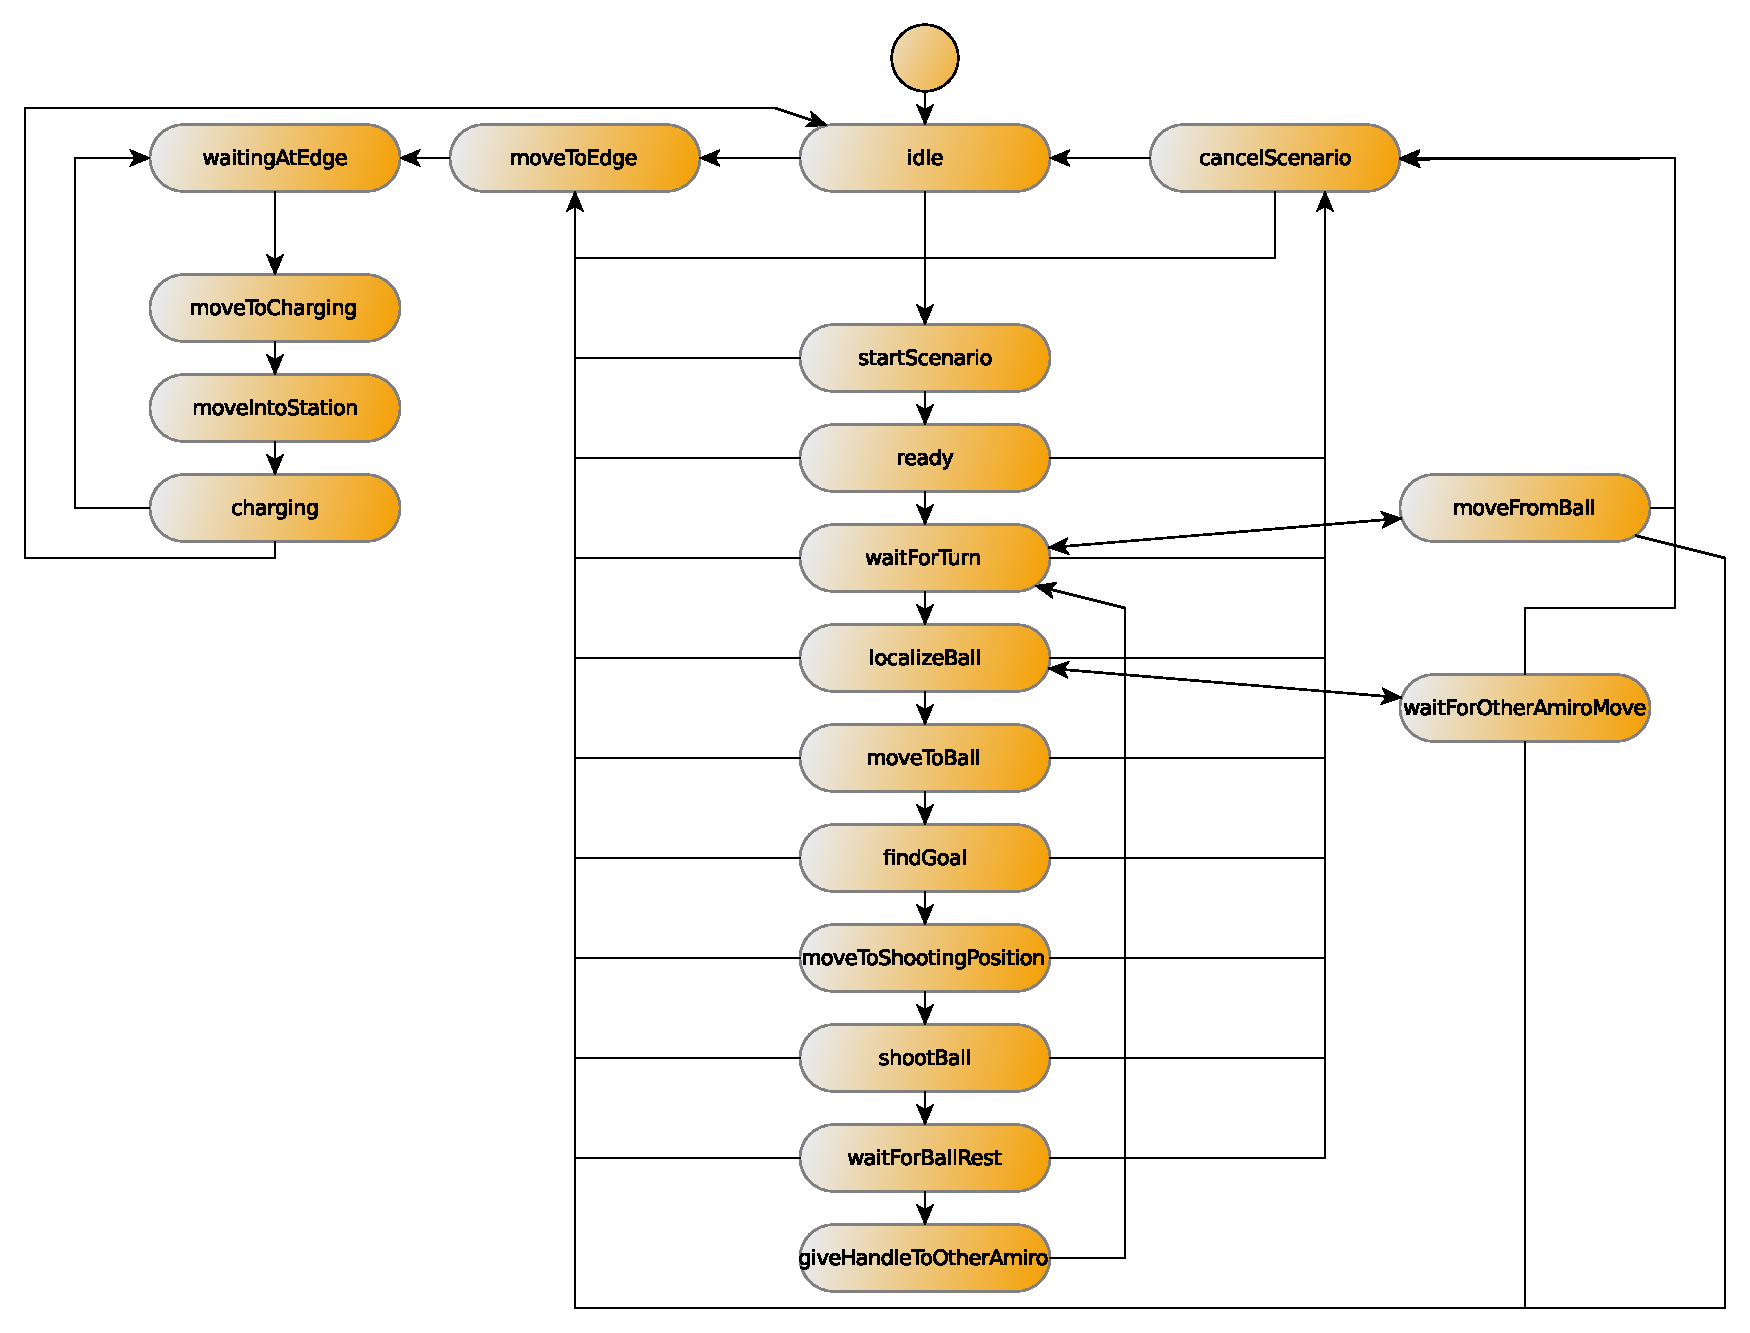
\includegraphics[scale=.55]{Final_FSM_AMiRo.pdf} 	
		\caption{Finite-State-Machine}
		\label{fig:fsm-amiro}
	\end{center}
\end{figure}
\begin{figure}
	\begin{center}
		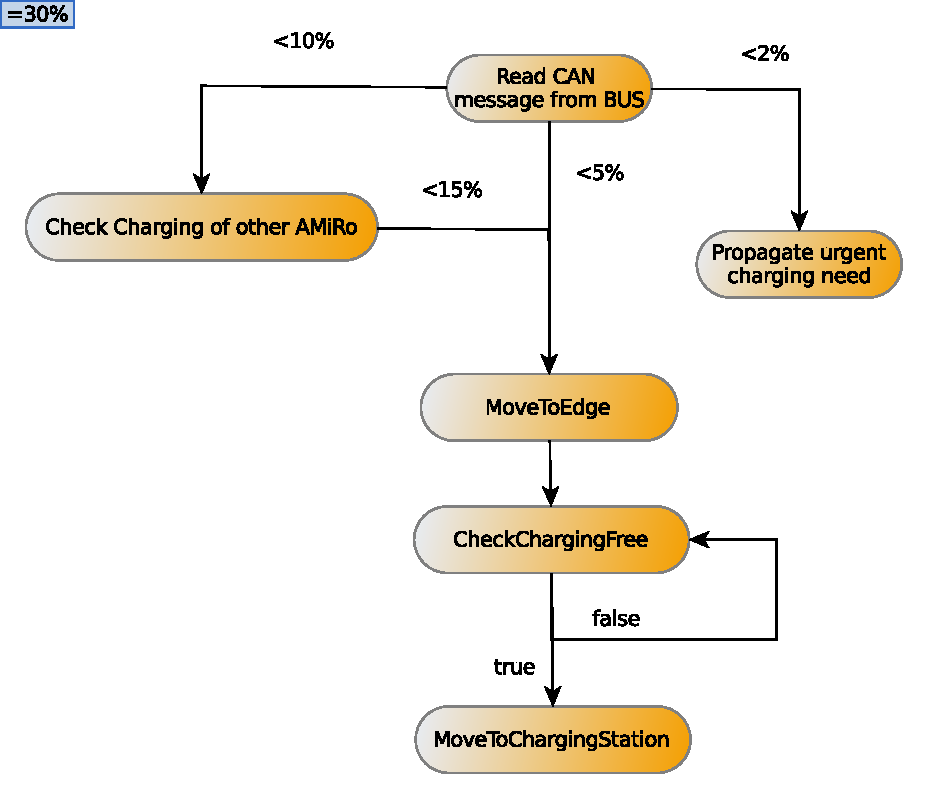
\includegraphics[scale=.50]{Charging_Strategy.pdf} 	
		\caption{Ladestrategie}
		\label{fig:charging-strategy}
	\end{center}
\end{figure}


\section[Realisierung der einzelnen Spielelemente]{Realisierung der einzelnen Spielelemente\hfill {\normalsize ?.?.}}%TODO: Besseren Sectiontitel

\subsection[Lokalisation des Balls]{Lokalisation des Balls\hfill {\normalsize J.E.}} %TODO: Julian E.

\subsection[Anfahren des Balls]{Anfahren des Balls\hfill {\normalsize J.E.}} %TODO: Julian E.

\subsection[Lokalisation des gegnerischen Tores]{Lokalisation des gegnerischen Tores\hfill {\normalsize T.M.}} %TODO: Timo M.

Nachdem der AMiRo an den Ball herangefahren ist beginnt er mit der Lokalisation des gegnerischen Tores. 
Hierfür fängt der Roboter an sich langsam gegen den Uhrzeigersinn um die eigene Achse zu drehen. Dabei wird der Rotationswinkel gespeichert und nach einer vollen Umdrehung wird die Drehung beendet. 
Während der Rotation werden die Bilder der Kamera darauf untersucht, ob die Torpfosten sichtbar sind. Die Detektion des Tores geschieht mittels des \textit{SimpleBlobDetector} der OpenCV-Programmbibliothek. Hierfür werden zunächst alle Pixel eines Bildes, die der Farbe des gegnerischen Tores entsprechen weiß und die restlichen schwarz eingefärbt.

Wenn ein einzelner Blob detektiert wurde, wird dessen Position gespeichert und die Rotation fortgesetzt. Sobald zwei Blobs im Bild detektiert wurden, wird die Rotation des AMiRos gestoppt, da das gegnerische Tor nun gefunden wurde. Zunächst wird der Winkel des Mittelpunkt des Tores zur vertikalen Mittelachse des Kamerabildes berechnet. Weiter wird der gespeicherte Rotationswinkel hinzu addiert, um den Winkel zwischen der Ausgangssituation und dem Tor zu erhalten. Dies ist der Winkel Theta ($\theta$), welcher in Abbildung \ref{fig:anfahren_schritt1} eingezeichnet ist. 
Sollte während einer vollen Rotation nur ein Pfosten detektiert werden, so wird der Winkel zu diesem berechnet.

Anschließend dreht der AMiRo sich wieder in Richtung des Balles. Der berechnete Winkel Theta wird der \textit{takeAim(..)}-Methode übergeben, die anschließend den AMiRo in seine Schussposition navigiert.

%- Rotation um eigene Achse zur Lokalisation des Tores
%- Lokalisation Anhand von Blobb-Detektion 
%- Wenn ein einzelner Pfosten im Bild vorhanden ist - bereits gedrehten Winkel + zusätlichen Winkel vom Mittelpunkt des Bildes zum Pfosten speichern
%- Wenn beide Pfosten im Bild vorhanden sind - bereits gedrehten Winkel + zusätlichen Winkel vom Mittelpunkt des Bildes zum Tormittelpunkt speichern und Rotation beenden
%- Drehung zum Ball durchführen, um diesen wieder vor sich zu haben

\subsection[Schussposition anfahren]{Schussposition anfahren\hfill {\normalsize T.M.}} %TODO: Timo M.

Zum Anfahren der Schussposition des AMiRos wird zunächst entschieden, ob der AMiRo den Ball im oder gegen den Uhrzeigersinn umfahren soll. Dies wird anhand des übergebenen Torwinkels entschieden. Ist dieser kleiner oder gleich 180$^\circ$, so wird der Ball gegen den Uhrzeigersinn umfahren, andernfalls im Uhrzeigersinn.
Nachdem dies entschieden wurde führt der AMiRo eine 90$^\circ$-Drehung in die gegebene Richtung aus. 
Nun umfährt der Roboter den Ball in einer kreisförmigen Bewegung so lange, bis der umfahrende Winkel dem Winkel zum Tor entspricht (siehe Abb. \ref{fig:anfahren_schritt1}). Danach dreht der AMiRo sich zurück zum Ball, welcher sich nun zwischen Roboter und Tor befindet.
Sollte während des Erreichen der Schussposition ein Hindernis im Weg sein, so wird die Bewegung gestoppt, eine Drehung zum Ball vollführt und diese Position für einen Schussversuch genutzt. Dieses Problem taucht vor allem auf, wenn der Ball zu nah an der Wand liegt.

Da bei der Berechnung des Winkels die Distanz zum Ball nicht mit eingerechnet wurde kann es nun der Fall sein, dass sich der Mittelpunkt des Tores nicht geradlinig vor dem AMiRo befindet. Hierfür wird nun abermals der Winkel des Tormittelpunkts zur vertikalen Achse des Kamerabildes berechnet und entschieden, ob die Position gut genug für einen Schuss ist, oder noch nachgebessert werden muss. 
Für das Nachjustieren wird die \textit{takeAim(..)}-Methode rekursiv aufgerufen, wobei der neue Winkel übergeben wird (siehe Abb. \ref{fig:anfahren_schritt2}). Zudem wird die Toleranz für die Position des Tores verdoppelt, um sicherzustellen, dass die Funktion nach einiger Zeit terminiert und nicht endlos versucht die Position des AMiRos zu verbessern.

\begin{figure} []
	\subfigure[Schritt 1]{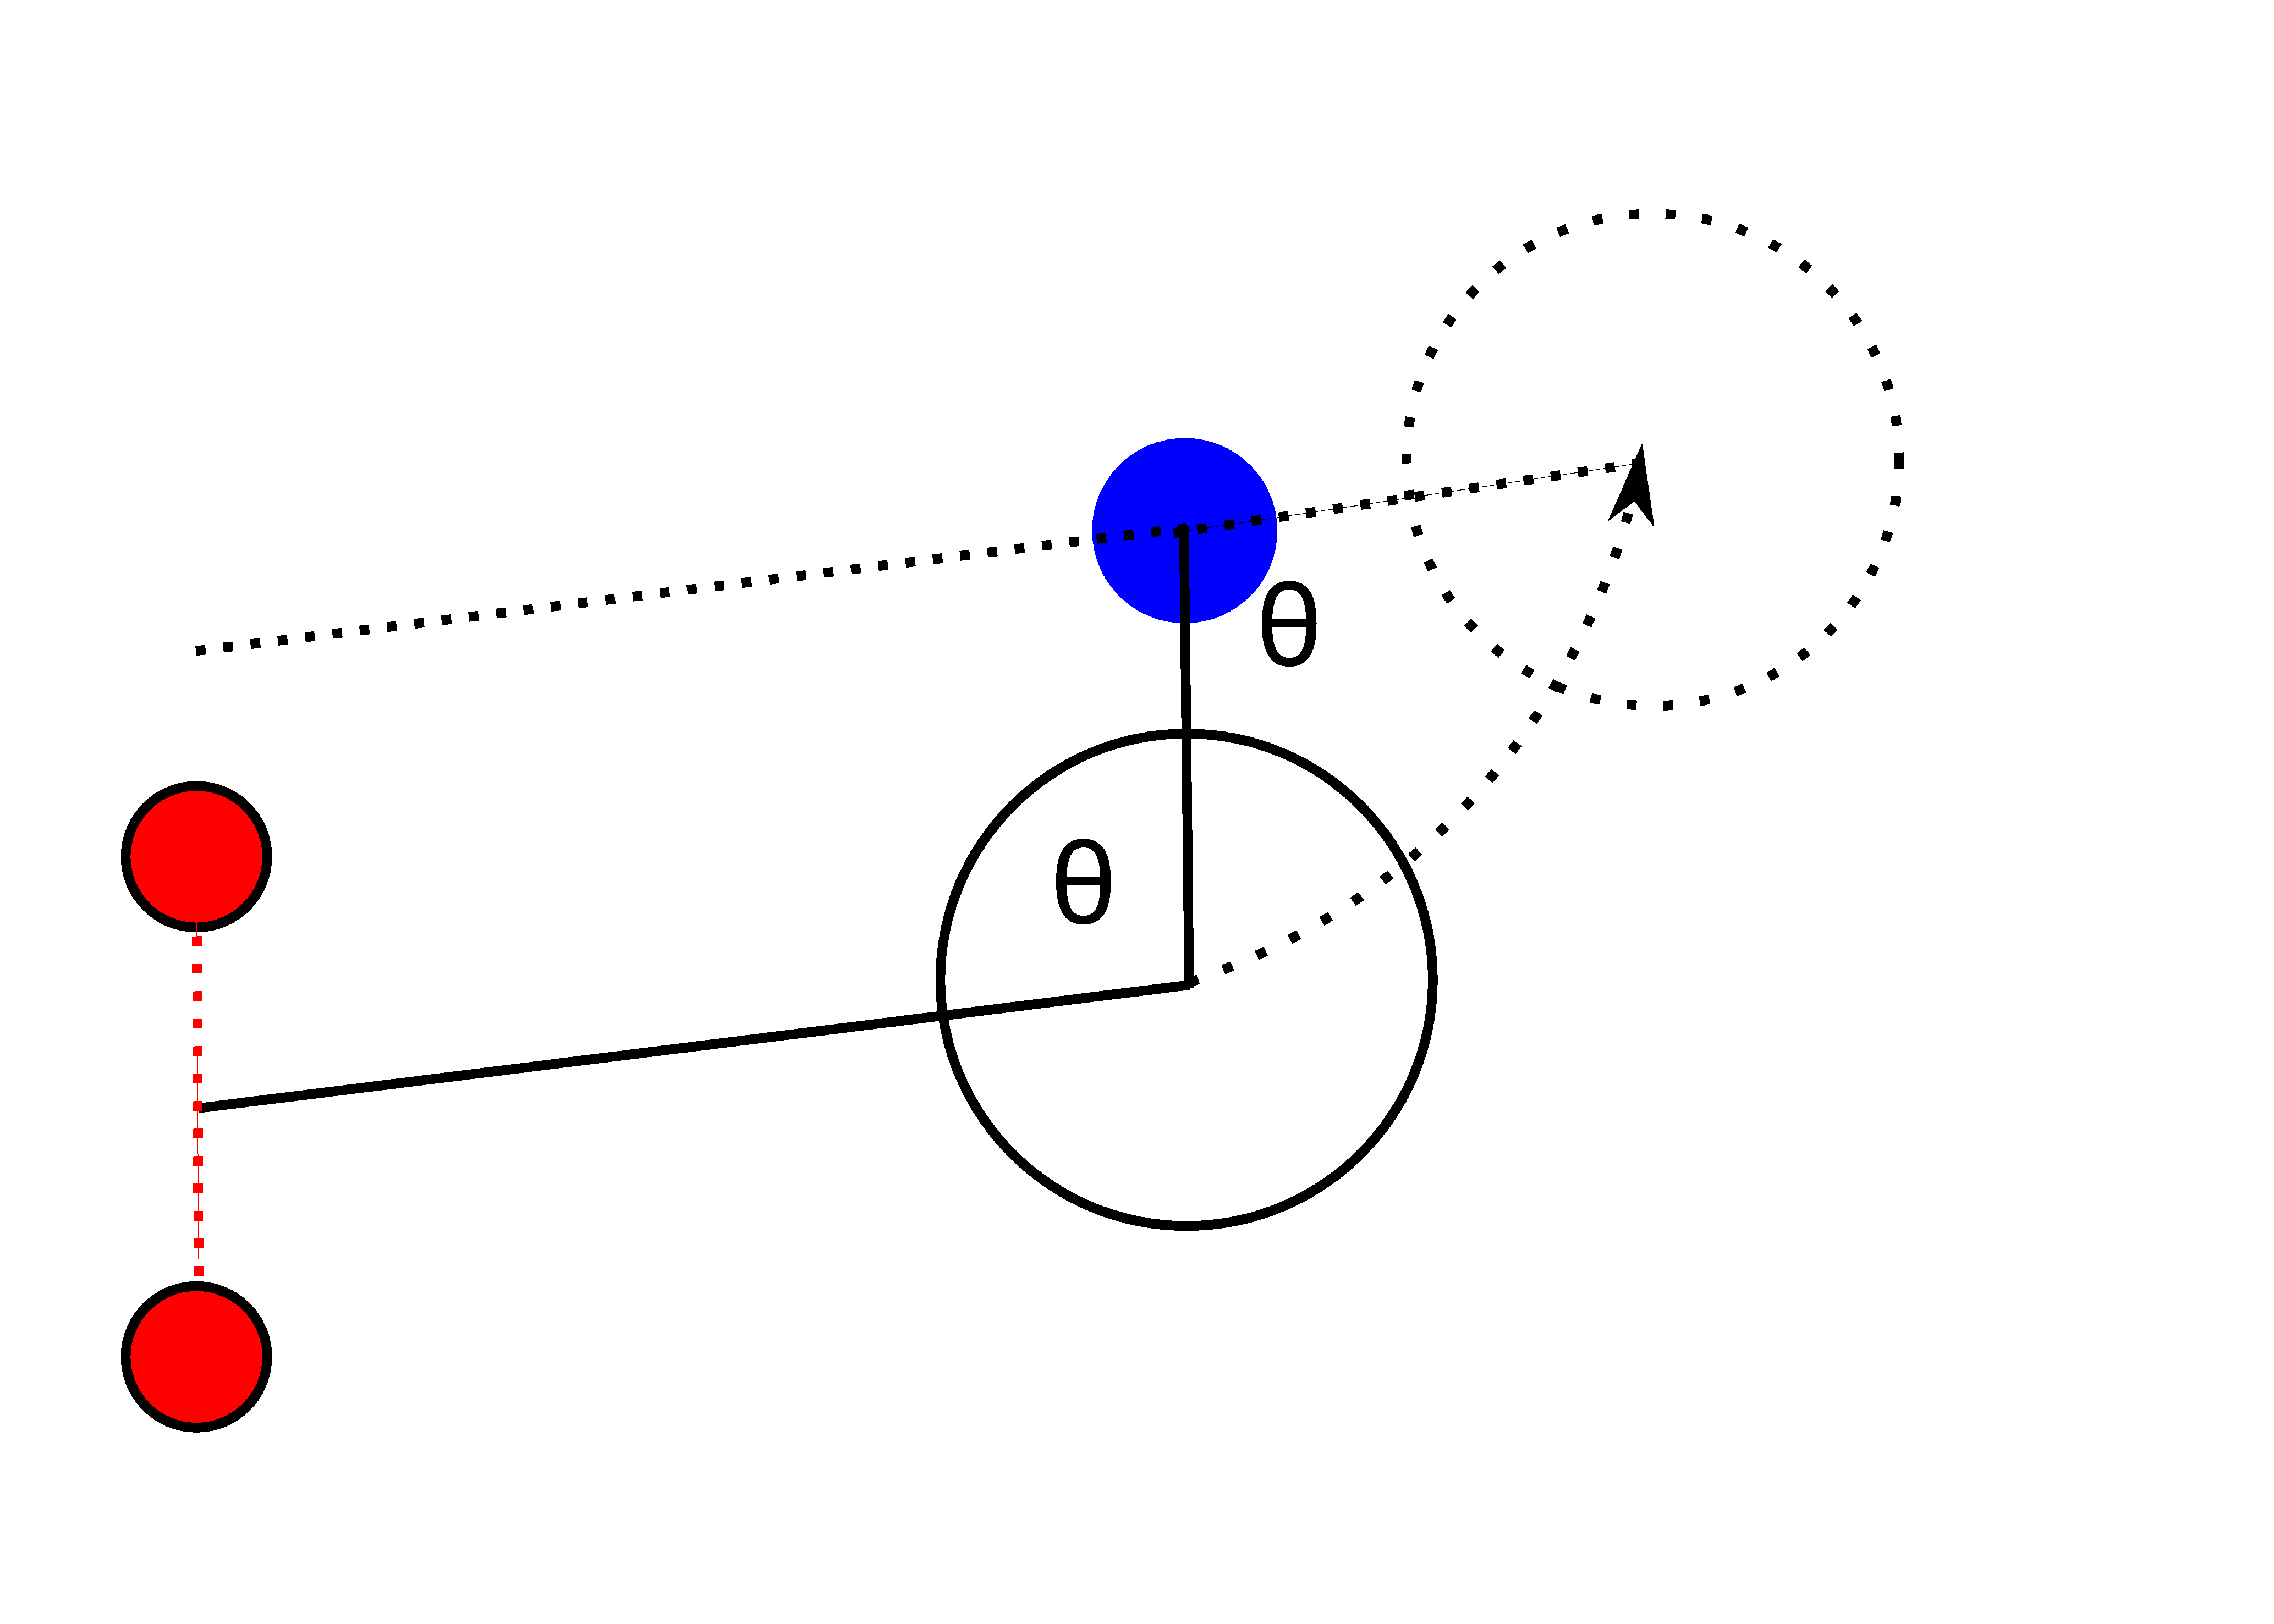
\includegraphics[width=0.45\textwidth]{takeaim1.pdf}\label{fig:anfahren_schritt1}} 
	\subfigure[Schritt 2]{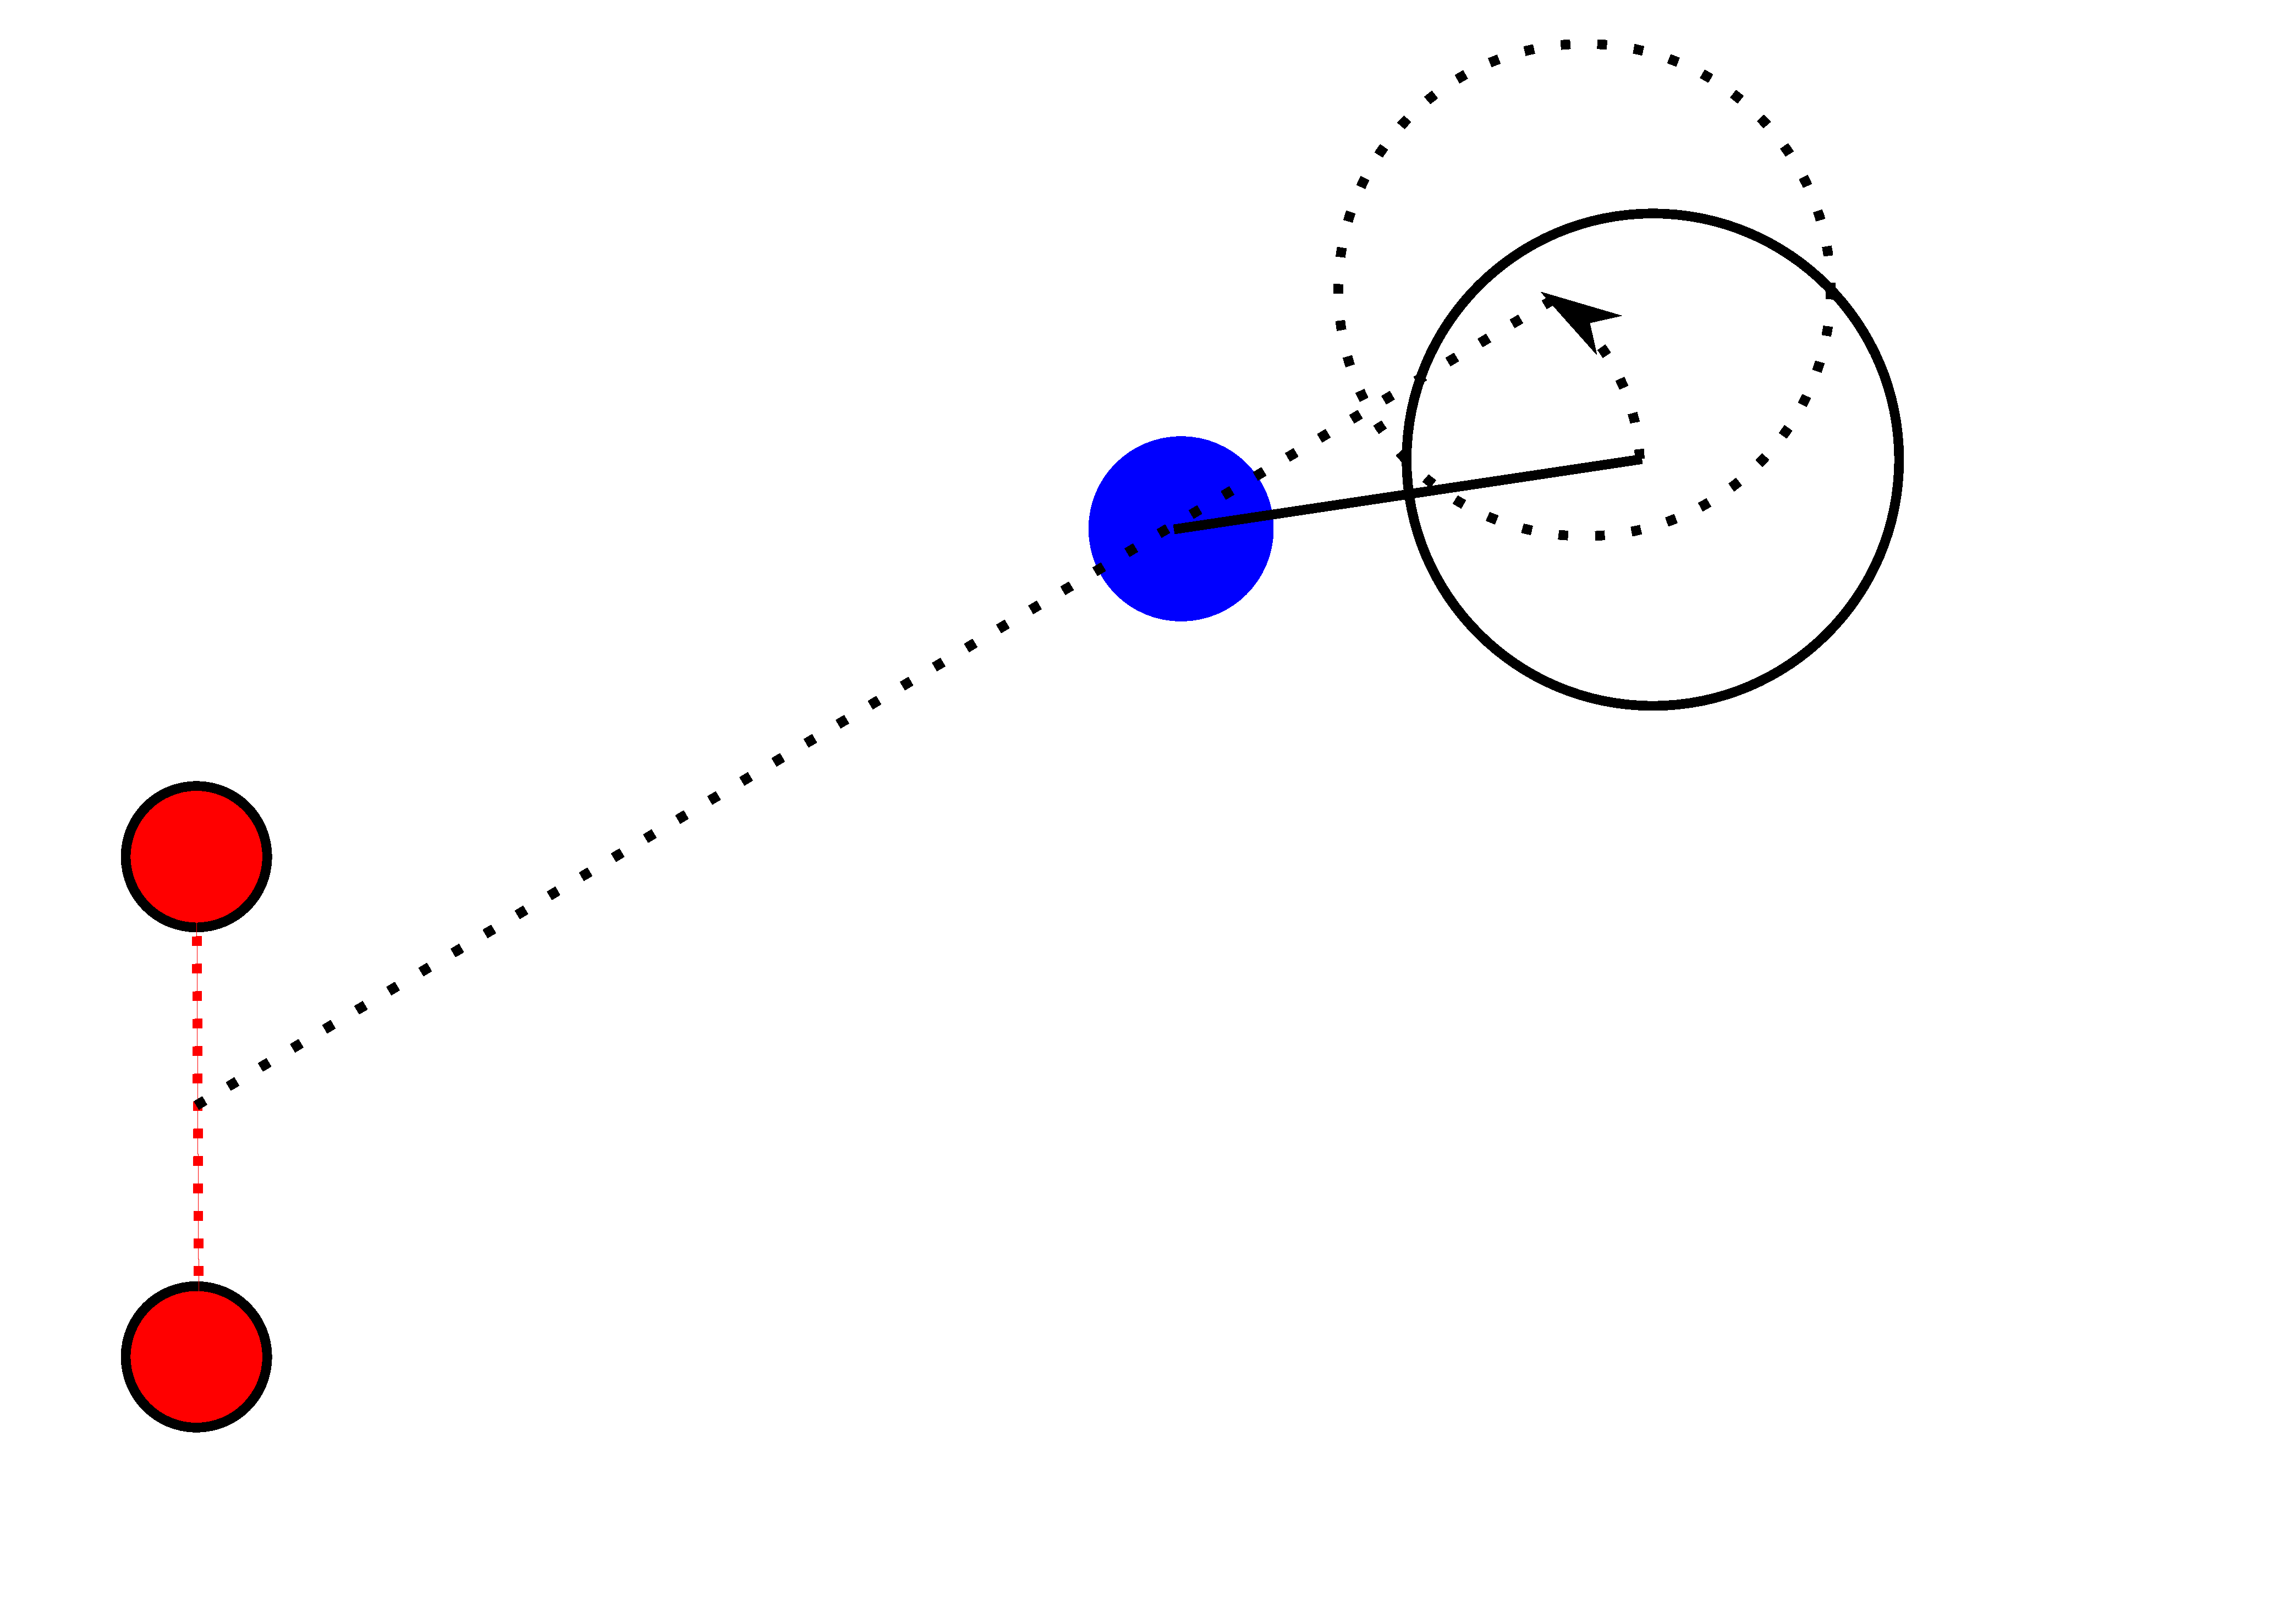
\includegraphics[width=0.45\textwidth]{takeaim2.pdf}\label{fig:anfahren_schritt2}} 
	\caption{Anfahren der Schussposition} 
	\label{fig:anfahren}
\end{figure} 

%- Je nach Winkel zum Tor entscheiden, ob der Ball links- oder rechtsseitig umfahren werden soll
%- 90$^\circ$ Drehung zu der gegebenen Seite 
%- Umfahren des Balles bis vorher berechneter Winkel zum Tor erreicht ist
%	- Bei einem Hindernis wird das Umfahren des Balles gestoppt
%- 90$^\circ$ Drehung zum Ball
%- Überprüfung, ob sowohl Ball als auch das Tor im Bild zu sehen ist 
%	- Ist dies der Fall -> feinjustierung der Schussposition 

\subsection[Schießen des Balles]{Schießen des Balles\hfill {\normalsize T.M.}} %TODO: Timo M.

Nachdem der AMiRo seine finale Schussposition erreicht hat wird die Funktion zum Schießen des Balles aufgerufen. Dabei werden zunächst die Sensorwerte der seitlichen Abstandssensoren darauf untersucht, ob der AMiRo sich zu nah an einer Wand befindet um einen geraden Schuss auszuführen. Die vorderen Abstandssensoren sind für diese Detektion nicht zu nutzen, da sich der Ball direkt vor dem AMiRo befindet und dieser als eine Wand fehlinterpretiert werden würde. 
Stellt der Roboter fest, dass sich keine Wand im Weg befindet, so führt er eine kurze schnelle Bewegung in Richtung des Balles aus um diesen zu schießen.
Sollte sich auf einer Seite des AMiRos eine Wand befinden, so führt er einen angedrehten Schuss aus, indem er bei der Bewegung zum Ball eine Kurve fährt, die den Roboter von der Wand hinweg dreht. 
Sollten sich auf beiden Seiten Wände befinden, so ist ein Schuss zu gefährlich, da der AMiRo gegen die Wand fahren würde.

%- Überprüfen der seitlichen vorderen Abstandssensoren ob eine Wand detektiert wird
%	- Sollte eine Wand auf einer Seite detektiert werden -> Angedrehter Schuss mit Drehung des AMiRos weg von der Wand
%- Schießen des Balles durch kurzes Ansteuern beider Motoren 

\subsection[Beiseite Fahren]{Beiseite Fahren\hfill {\normalsize J.E.}} %TODO: Julian E.

\subsection[Torjubel]{Torjubel\hfill {\normalsize A.G.}} %TODO: Andi G.

\section[Externes Spieltracking]{Externes Spieltracking\hfill {\normalsize J.D.}} %TODO: Julian D.

Zusätzlich zu den beiden AMiRos, die in dem Fußballszenario agieren, sorgt ein zusätzlicher Host-PC für die Koordination des Spielablaufs. Dazu kommuniziert auch er, wie bereits in Kapitel \ref{sec:szenario_koordination} beschrieben, über eine RSB-/Spreadverbindung sowohl intern über zwei Prozesse hinweg, als auch extern zu den AMiRos. Zusätzlich ist eine handelsübliche Webcam in einem geneigten Winkel rund 2 Meter über dem Spielfeld angebracht, um die Erkennung und Aufbereitung entscheidender Spielelemente mithilfe von Bildverarbeitungsverfahren ermöglichen zu können.

Die beiden intern kommunizierenden Prozesse lauten \texttt{localizationShowcase} und \texttt{processShowcase}. Während \texttt{localizationShowcase} das Kamerabild abgreift und die Detektion von Markern übernimmt, analysiert \texttt{processShowcase} das Spielgeschehen mithilfe einer Blobdetektion und zeigt zudem die grafische Benutzeroberfläche an. Neben dem Vorteil der besseren Wartbarkeit, ist der Grund für die Unterteilung in zwei seperate Prozesse die Unvereinbarkeit der verwendeten Softwarebibliotheken ARToolKit und OpenCV.

\subsection[Markerdetektion mit dem ARToolKit]{Markerdetektion mit dem ARToolKit\hfill {\normalsize J.D.}} %TODO: Julian D.

Das ARToolKit ist eine Open-Source-basierte Softwarebibliothek, die aus dem Bereich der Augmented Reality stammt. Während die möglichen Anwendungsszenarien des ARToolKits vielzählig sind, liegt eine seiner Kernkompetenzen in der schnellen sowie zuverlässigen Detektion und Lokalisation von vordefinierten Markern in einem Videostream. Beispiele für die verwendeten Marker sind in Abbildung \ref{fig:art_marker} dargestellt. Die Detektion erfolgt dabei sowohl rotations- als auch translationsinvariant und liefert dem Benutzer eine Bildkoordinate sowie einen Rotationswinkel.

\begin{figure}
	\begin{center}
		\subfigure{
			
\includegraphics[width=0.30\textwidth]{15.pdf}
		}
		\subfigure{
			
\includegraphics[width=0.30\textwidth]{17.pdf}
		}
		\subfigure{
			
\includegraphics[width=0.30\textwidth]{25.pdf}
		}
		\caption{Beispiele für Marker des ARToolKits}
		\label{fig:art_marker}
	\end{center}
\end{figure}

Abbildung \ref{fig:marker_detection} ist ein Beispielbild der verwendeten Webcam und es zeigt die Anwendungsgebiete der Markerdetektion im Rahmen des Fußballszenarios. Zum einen sind vier Marker in den jeweiligen Eckpunkten des Schaukastens angebracht. Anhand dessen soll im weiteren Verlauf eine Vorselektierung des Bildausschnittes ermöglicht werden um die Bildverarbeitung zum Einen beschleunigen und zum Anderen die Fehldetektion von Objekten außerhalb des Glaskastens verhindern zu können. Außerdem befinden sich Marker auf der Oberseite der AMiRos. Diese haben im aktuellen Zustand keinen praktischen Nutzen für die Spielmechanik an sich, ermöglichen es der grafischen Benutzeroberfläche aber, die aktuelle Position der AMiRos ansprechend zu visualisieren. Zusätzlich sind einige Marker auf DIN A4 Papier aufgetragen. Diese lösen auf dem Host-PC vordefinierte Events aus und ermöglichen dem Anwender dadurch eine direkte Interaktion ohne die Zuhilfenahme von klassischen Eingabegeräten wie Maus oder Tastatur.

\begin{figure}
	\begin{center}
		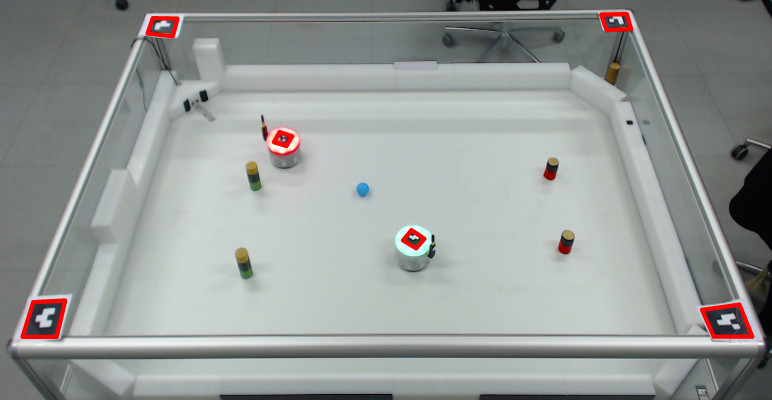
\includegraphics[width=\textwidth]{marker_detection.jpg} 	
		\caption{Detektion der ARToolKit Marker}
		\label{fig:marker_detection}
	\end{center}
\end{figure}

Die Einbettung des ARToolKits wird im Rahmen dieses Projektes durch das Programm \texttt{localizationShowcase} realisiert. Dieses bedient sich zunächst der Videoschnittstelle Video4Linux um die Bilddaten der Webcam abzugreifen. In einem nächsten Schritt wird eine neue Instanz des RSB-Datentyps \texttt{trackingImage} angelegt. Der Prototyp dieses Datentyps beinhaltet sowohl den Standardtyp \texttt{Image} aus der RSB-Bibliothek, als auch eine Liste von Elementen des Typs \texttt{Pose2D} welche jeweils die Felder \texttt{X}, \texttt{Y}, \texttt{orientation} und \texttt{id} beinhalten. Die Kombination dieser beiden Typen bringt den Vorteil mit sich, dass Bild- und Trackingdaten bereits synchronisiert auf der Seite des Empfängers ankommen, ohne dass dieser weitere Ressourcen für die Synchronisation benötigen würde.

Für jedes abgegriffene Videobild wird also ein \texttt{trackingImage}-Objekt erzeugt, welches zusätzlich zum unveränderten Kamerabild eine Liste von erfolgreichen Markerdetektionen beinhaltet. Dieses Objekt wird anschließend über einen frei konfigurierbaren RSB-Scope an den zweiten Prozess des Host-PCs gesendet.

\subsection[Extraktion wichtiger Spielelemente mit Bildverarbeitungsmethoden]{Extraktion wichtiger Spielelemente mit Bildverarbeitungsmethoden\hfill {\normalsize J.D.}} %TODO: Julian D.
\begin{figure}
	\begin{center}
		\subfigure[Marker 1]{
			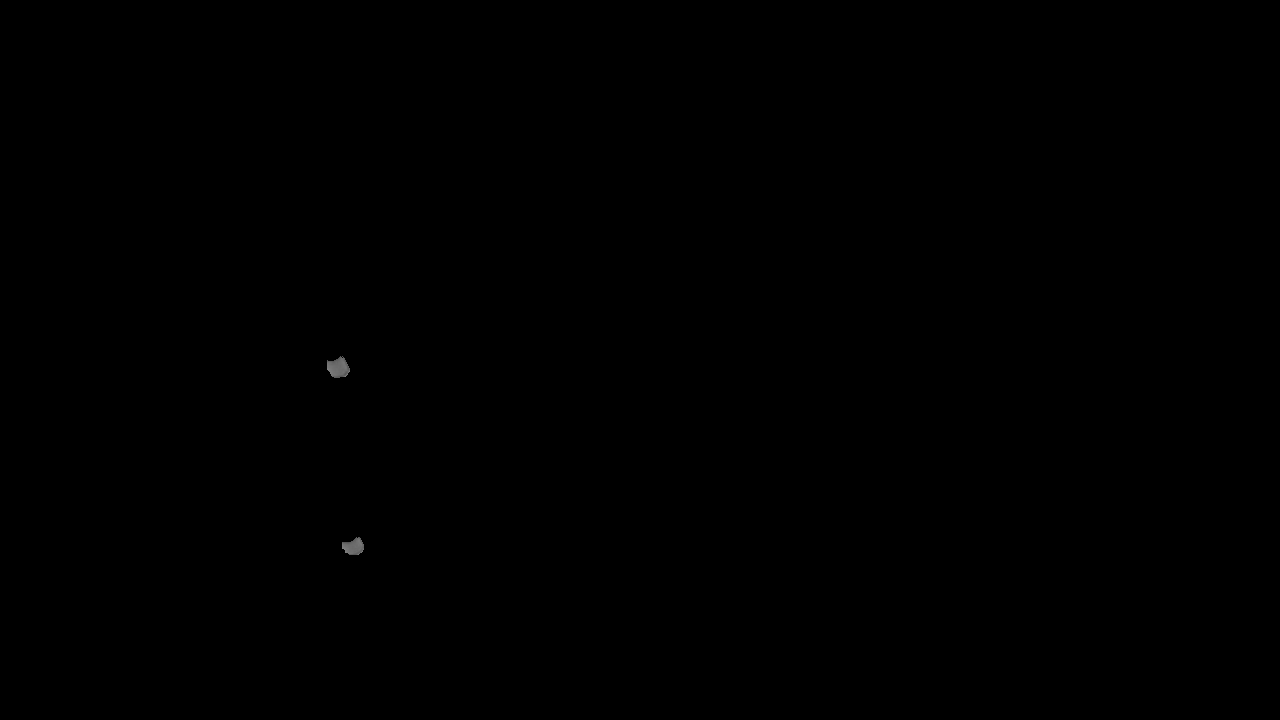
\includegraphics[width=0.31\textwidth]{blob_green.png}
			\label{fig:blob_green}
		}
		\subfigure[Marker 2]{
			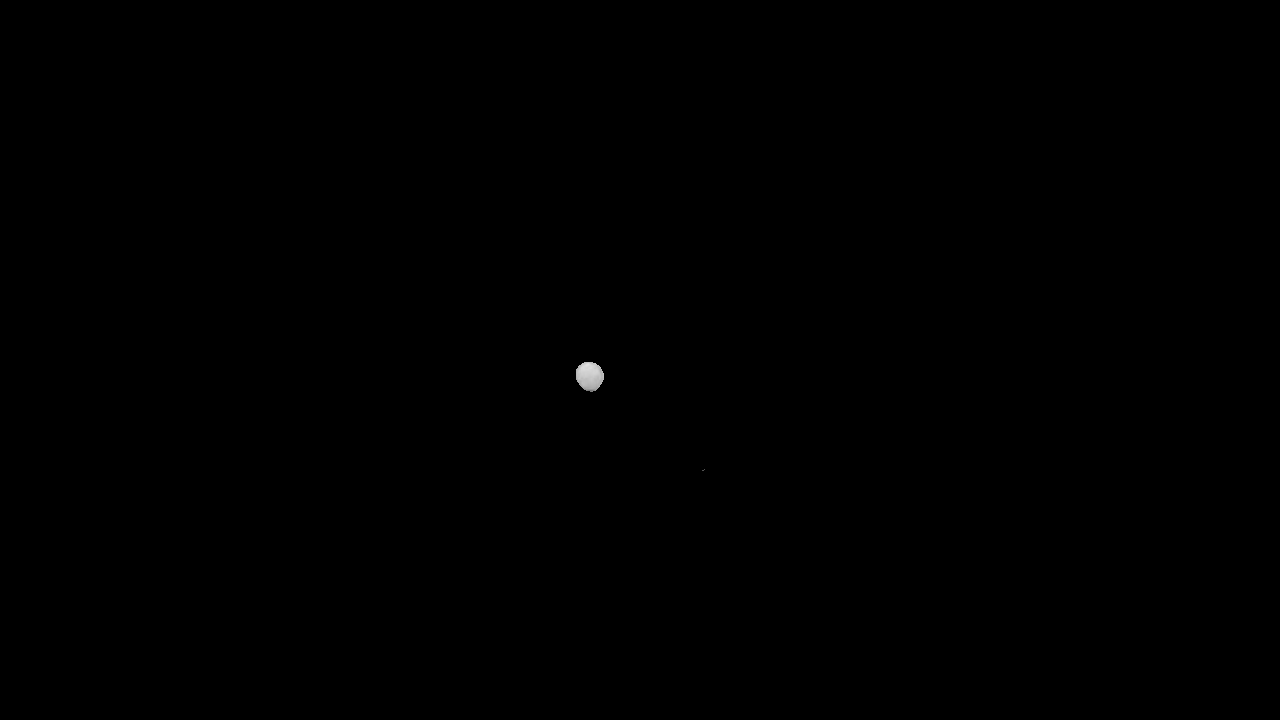
\includegraphics[width=0.31\textwidth]{blob_blue.png}
			\label{fig:blob_blue}
		}
		\subfigure[Marker 3]{
			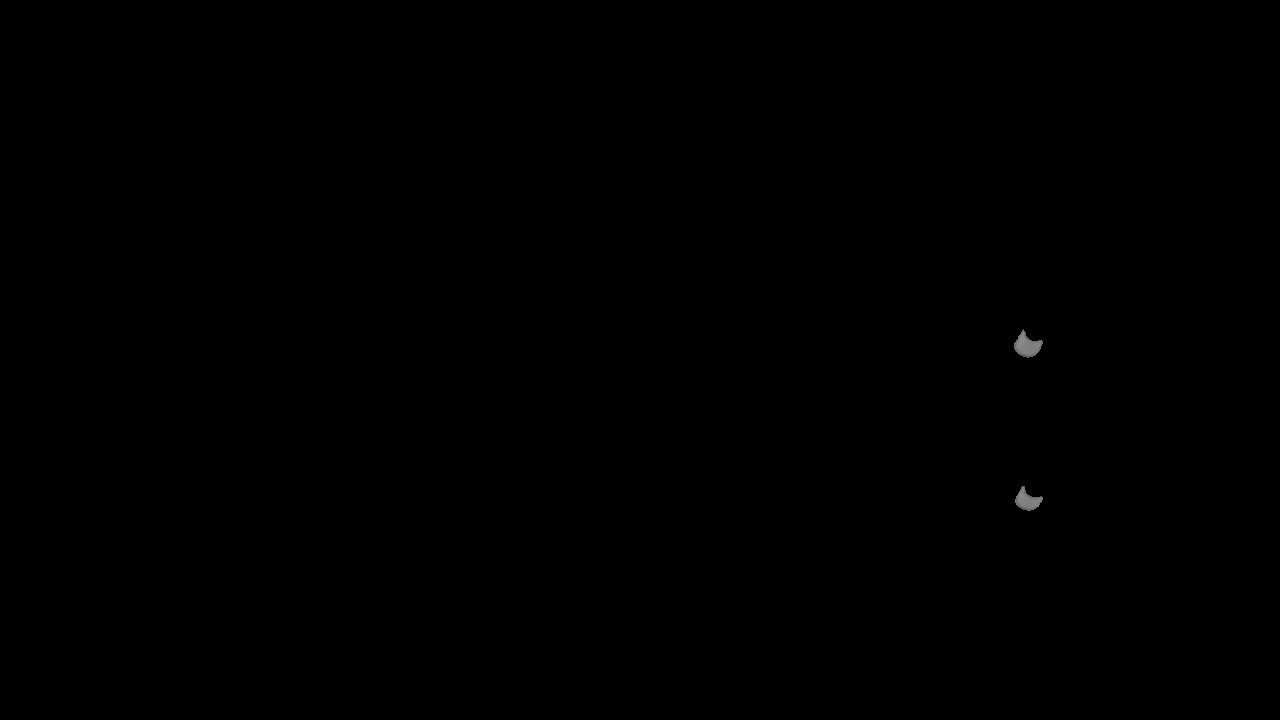
\includegraphics[width=0.31\textwidth]{blob_red.png}
			\label{fig:blob_red}
		}
		\caption{Verwendung der Blobdetektion}
	\end{center}
\end{figure}

\subsection[Spielkoordination]{Spielkoordination\hfill {\normalsize J.D.}} %TODO: Julian D.
\begin{figure}
	\begin{center}
		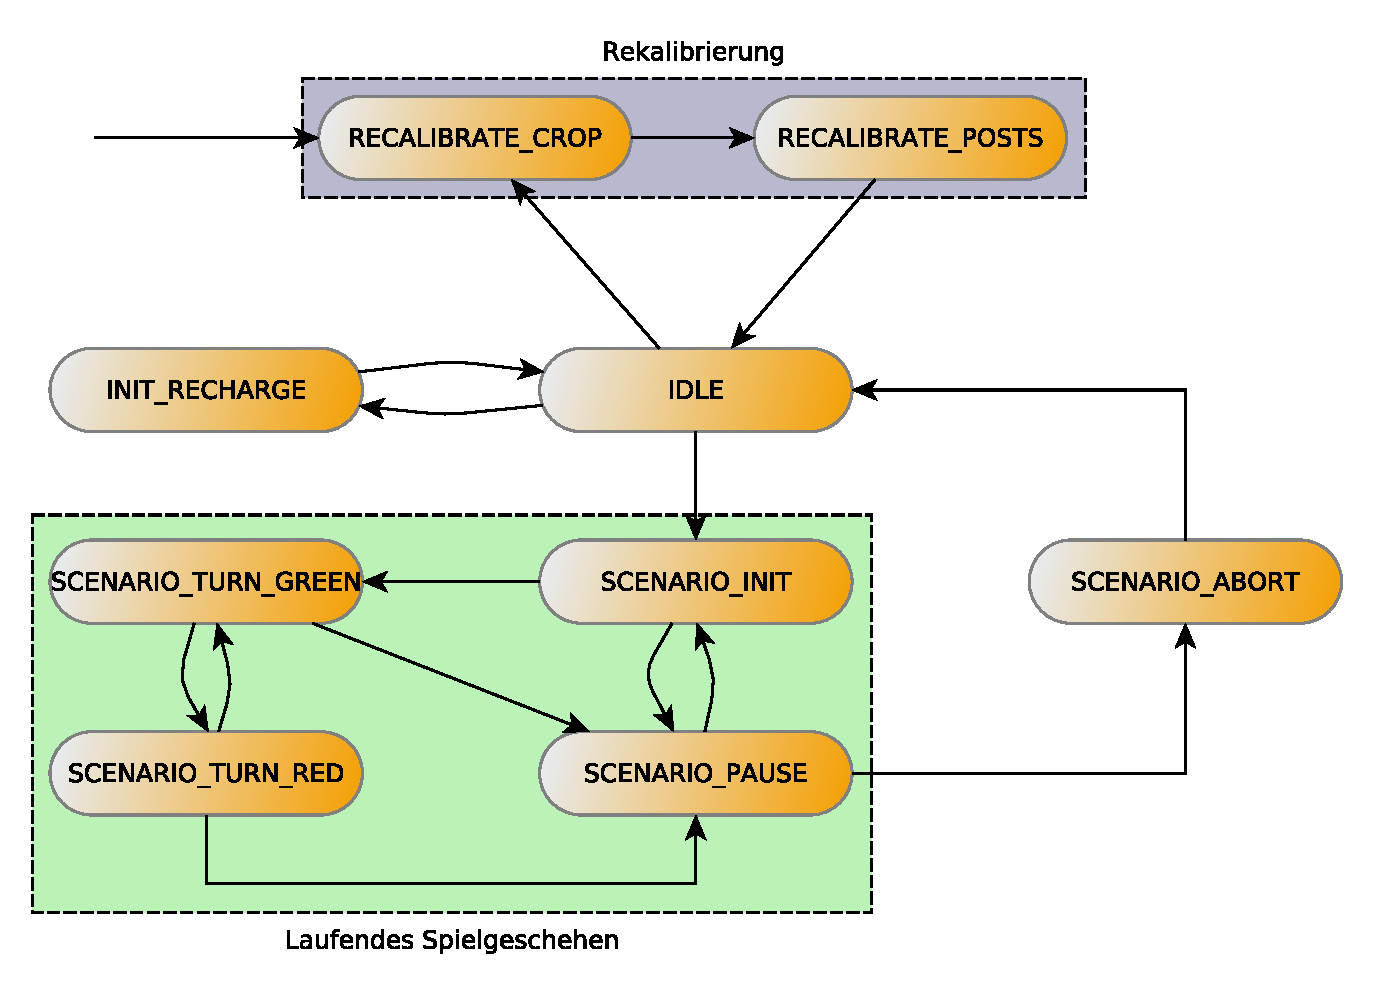
\includegraphics[width=\textwidth]{Tracking_FSM.pdf} 	
		\caption{FSM auf Host-Seite}
		\label{fig:fsm-host}
	\end{center}
\end{figure}

\subsection[Grafische Darstellung des Spielstatus]{Grafische Darstellung des Spielstatus\hfill {\normalsize J.D.}} %TODO: Julian D.

\begin{figure}
	\begin{center}
		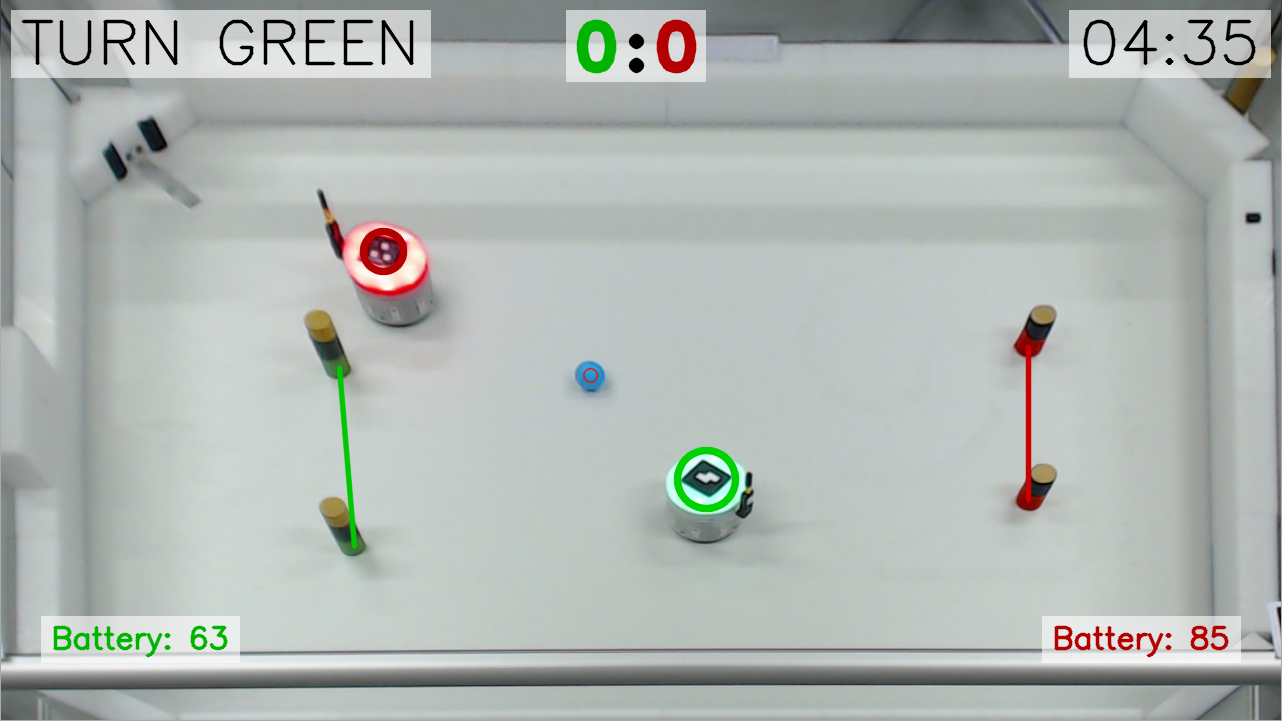
\includegraphics[width=\textwidth]{gui.png} 	
		\caption{Grafische Benutzeroberfläche}
		\label{fig:gui}
	\end{center}
\end{figure}
